\cleardoublepage
\section{\secState{R}Reduced Reach Sets Performance}\label{sec:reducedReachSetPerformance}

\noindent \emph{Constrained Expansion Method} (alg. \ref{alg:Wavefront Propagation}) is creating \emph{Reach Sets} from \emph{Root Node} as a tree expansion using \emph{Expansion Constraint function} (depending on type).

The \emph{Reach set creation procedure} is creating following artifacts:
\begin{enumerate}
    \item \emph{Nodes} - tree Node containing necessary data for discrete Trajectory portion, notably \emph{System State Evolution}, \emph{buffer}, and, \emph{Reachibility Rating}.
    
    \item \emph{Trajectories} - leaf \emph{Node} containing \emph{unique buffer} which is not \emph{prefix} in others Node buffer. 
\end{enumerate}

The \emph{Reach Set Computation Time} is depending strongly on \emph{Movement Automaton} prediction complexity and Node count. The \emph{Constrained Expansion Method} (alg. \ref{alg:Wavefront Propagation}) is separating all nodes entering into $cell_{i,j,k}$ into two distinctive groups: \emph{Candidates for expansion} and \emph{Leftover Nodes}. 

The \emph{Leftover Nodes} are thrown away every expansion. The \emph{Leftover Nodes} are not expanded in next \emph{Wave-front} iteration, but they leave a notable \emph{computation} and \emph{memory} footprint.

\begin{note}
    \emph{Average Trajectory Smoothness Rate} (def. \ref{def:SmoothnessRatingForTrajectory}) is important only in \emph{Navigation Mode}, this aspect has been covered over (sec. \ref{s:harmonicReachSet}, \ref{s:combinedReachSet}, \ref{s:acasReachSet}).
\end{note}

\paragraph{Approach:} For exactly same conditions (\emph{Testing Avoidance Grid}, \emph{UAS initial state}, \emph{Movement Automaton}) compare performance of \emph{Reach Set Approximations} created by various methods for following parameters:

\begin{enumerate}
    \item\emph{Coverage Ratio} - defined in (def. \ref{def:coverageRatio}) shows how versatile \emph{Reach Set Approximation} is (up to 100\% of complete reach set coverage). 
    
    \item\emph{Node count} - count of Nodes in \emph{Reach Set Approximation} counted like:
    \begin{enumerate}[a.]
        \item full -  all active nodes existing over computation time,
        \item pruned - active nodes for real time use.
    \end{enumerate}
    
    \item\emph{Count of Trajectories} - count of Trajectories (leaf Nodes) counted like:
    \begin{enumerate}[a.]
        \item full -  all active trajectories existing over computation time,
        \item pruned - active trajectories leading to coating cells of \emph{Avoidance Grid}.
    \end{enumerate}
\end{enumerate}


\paragraph{Testing Avoidance Grid}  with \emph{Distance 10 m}, \emph{Layer count 10}, \emph{Horizontal range $[-45^\circ,+45^\circ]$}, \emph{Horizontal Cell Count 7}, \emph{Vertical range $[-30^\circ,+30^\circ]$}, and \emph{Vertical Cell Count 5}. 

\begin{note}
    The sizing of \emph{Avoidance Grid} was chosen small scale, because property of \emph{Coverage Ratio} can be calculated exactly up to some scale, after that it can be only assumed. Various sizes of \emph{Avoidance Grid} was tested in \cite{gomola2017probabilistic}.
\end{note}

The UAS is at \emph{Back-side} of \emph{Figure} (initial state is at all \emph{Trajectory Origins}). The \emph{black dashed line} marks \emph{Avoidance Grid} space boundary. Each trajectory has its own color and ends at \emph{Front-side} of \emph{Avoidance Grid Boundary}.

\paragraph{Chaotic Reach Set} (sec. \ref{s:chaoticReachSet}) is used in \emph{Emergency Avoidance Mode} for \emph{Non-Controlled Airspace}. The \emph{full} set of trajectories is given in (fig. \ref{fig:chaoticComputed}). The \emph{Pruned} set of trajectories is given in (fig. \ref{fig:chaoticPruned}).

\emph{Tuning parameters} were selected like follow: \emph{Spread Ratio} is 15 (unique footprint trajectories in cell) and \emph{trajectory footprint length} is $3$ (last three unique passing cells). 


\begin{figure}[H]
    \centering
    \begin{subfigure}{0.48\textwidth}
    	\centering
        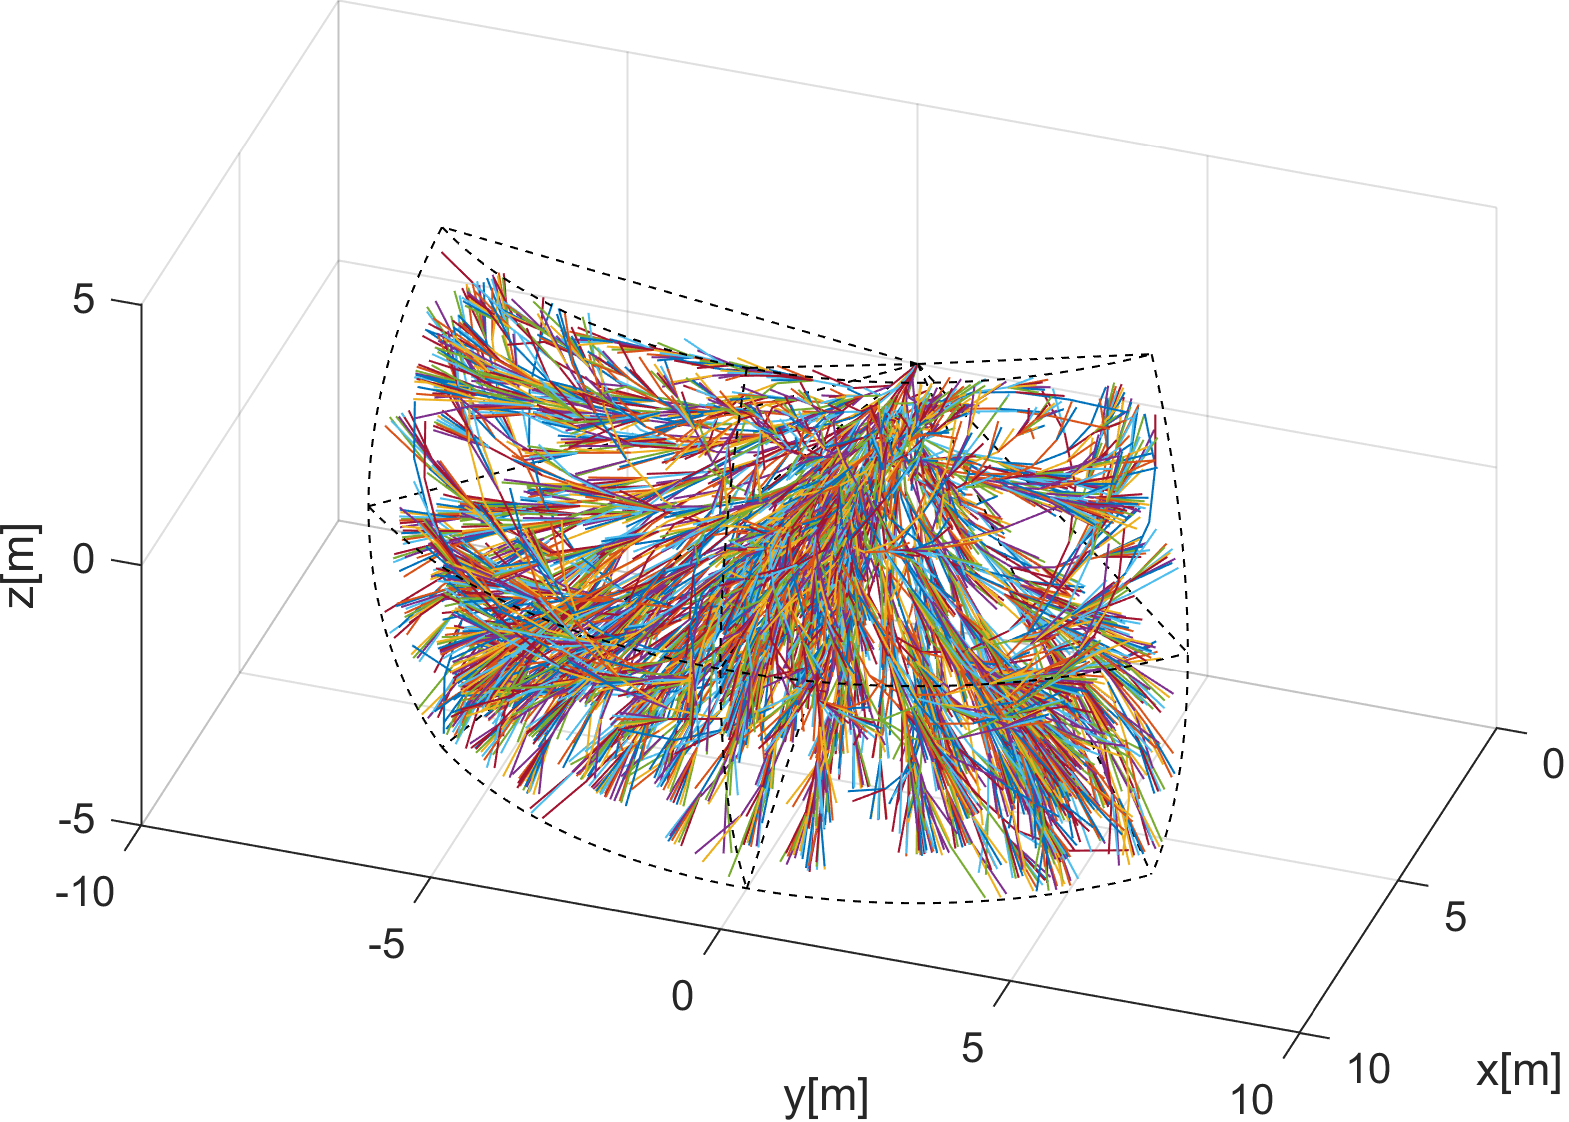
\includegraphics[width=0.9\linewidth]{\FIGDIR/NS082CoverageRS00010}
        \caption{Full.}
        \label{fig:chaoticComputed}
    \end{subfigure}
    \begin{subfigure}{0.48\textwidth}
    	\centering
        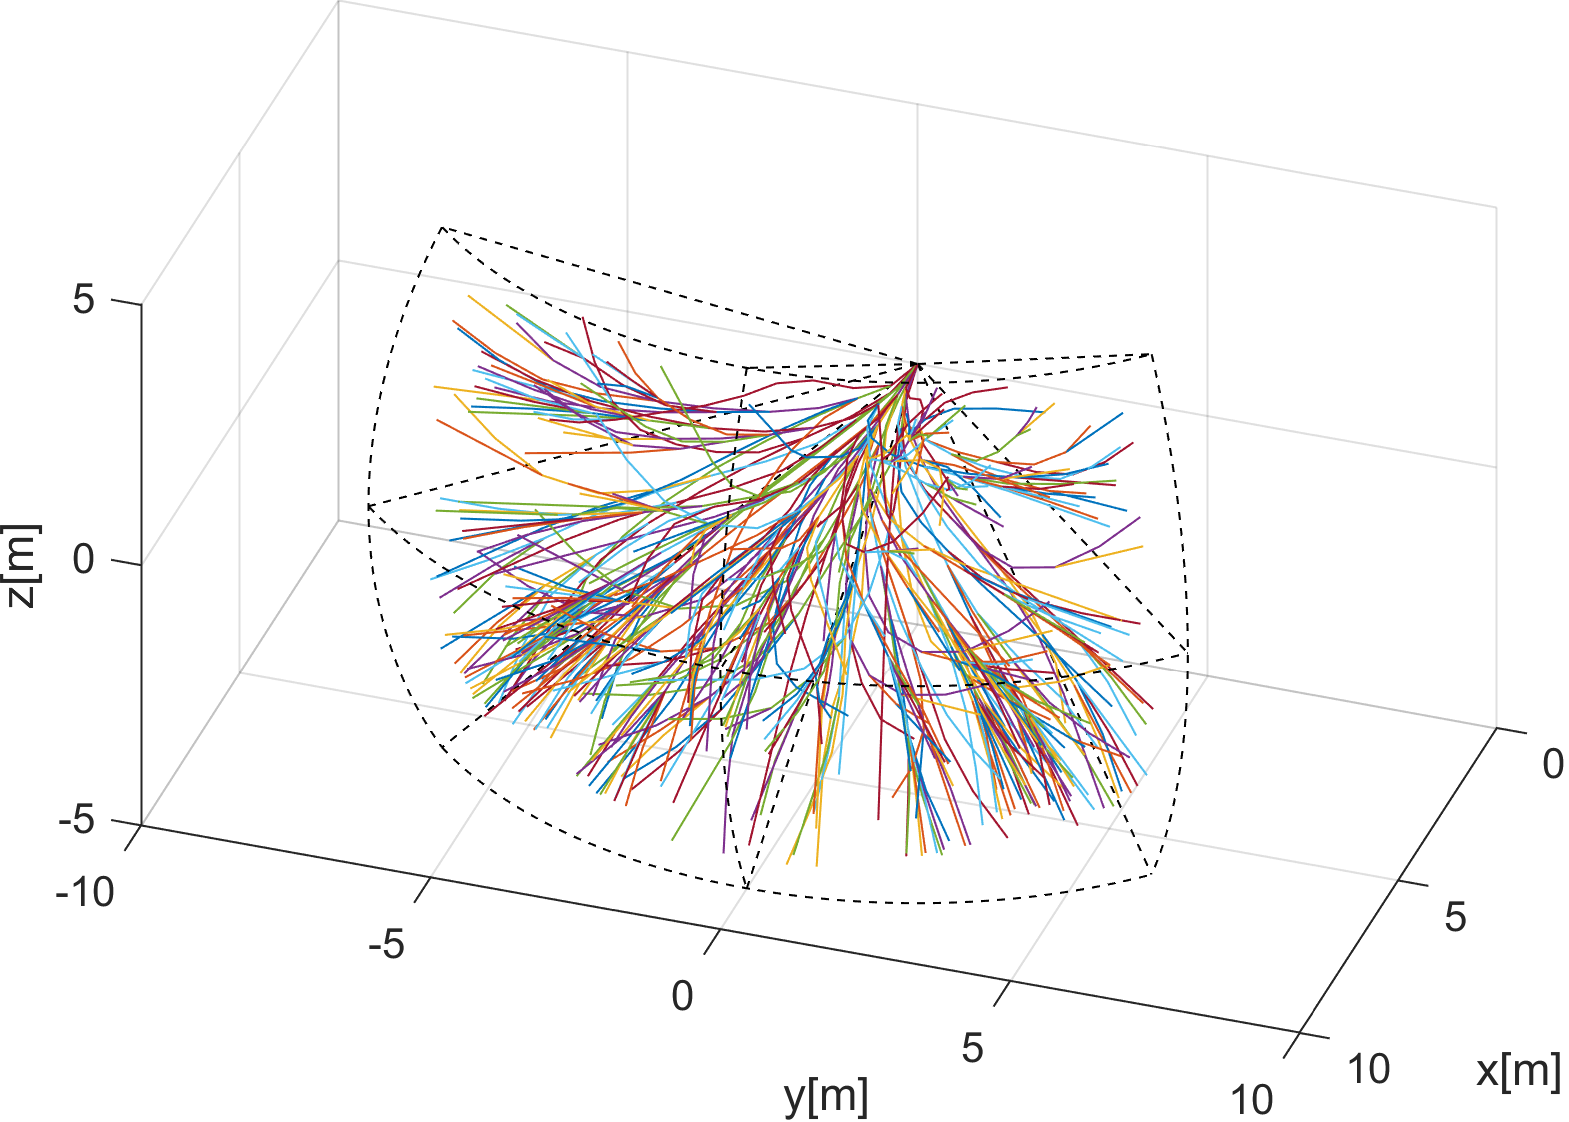
\includegraphics[width=0.9\linewidth]{\FIGDIR/NS083CoverageRSAfterPruning} 
        \caption{Pruned.}
        \label{fig:chaoticPruned}
    \end{subfigure}
    \caption{Chaotic reach set computation example.}
    \label{fig:chaoticReachSetComputationExample}
\end{figure}

\paragraph{Harmonic Reach Set} (sec. \ref{s:harmonicReachSet}) is used in \emph{Navigation Mode} for \emph{Non Controlled Airspace}. The \emph{full set} of trajectories is given in (fig. \ref{fig:harmonicComputed}). The \emph{Pruned} set of trajectories is given in (fig. \ref{fig:harmonicPruned}).

\emph{Tuning parameter} for \emph{harmonic spread ratio} was set to 9 (which implies high coverage).

\begin{figure}[H]
    \centering
    \begin{subfigure}{0.48\textwidth}
    	\centering
        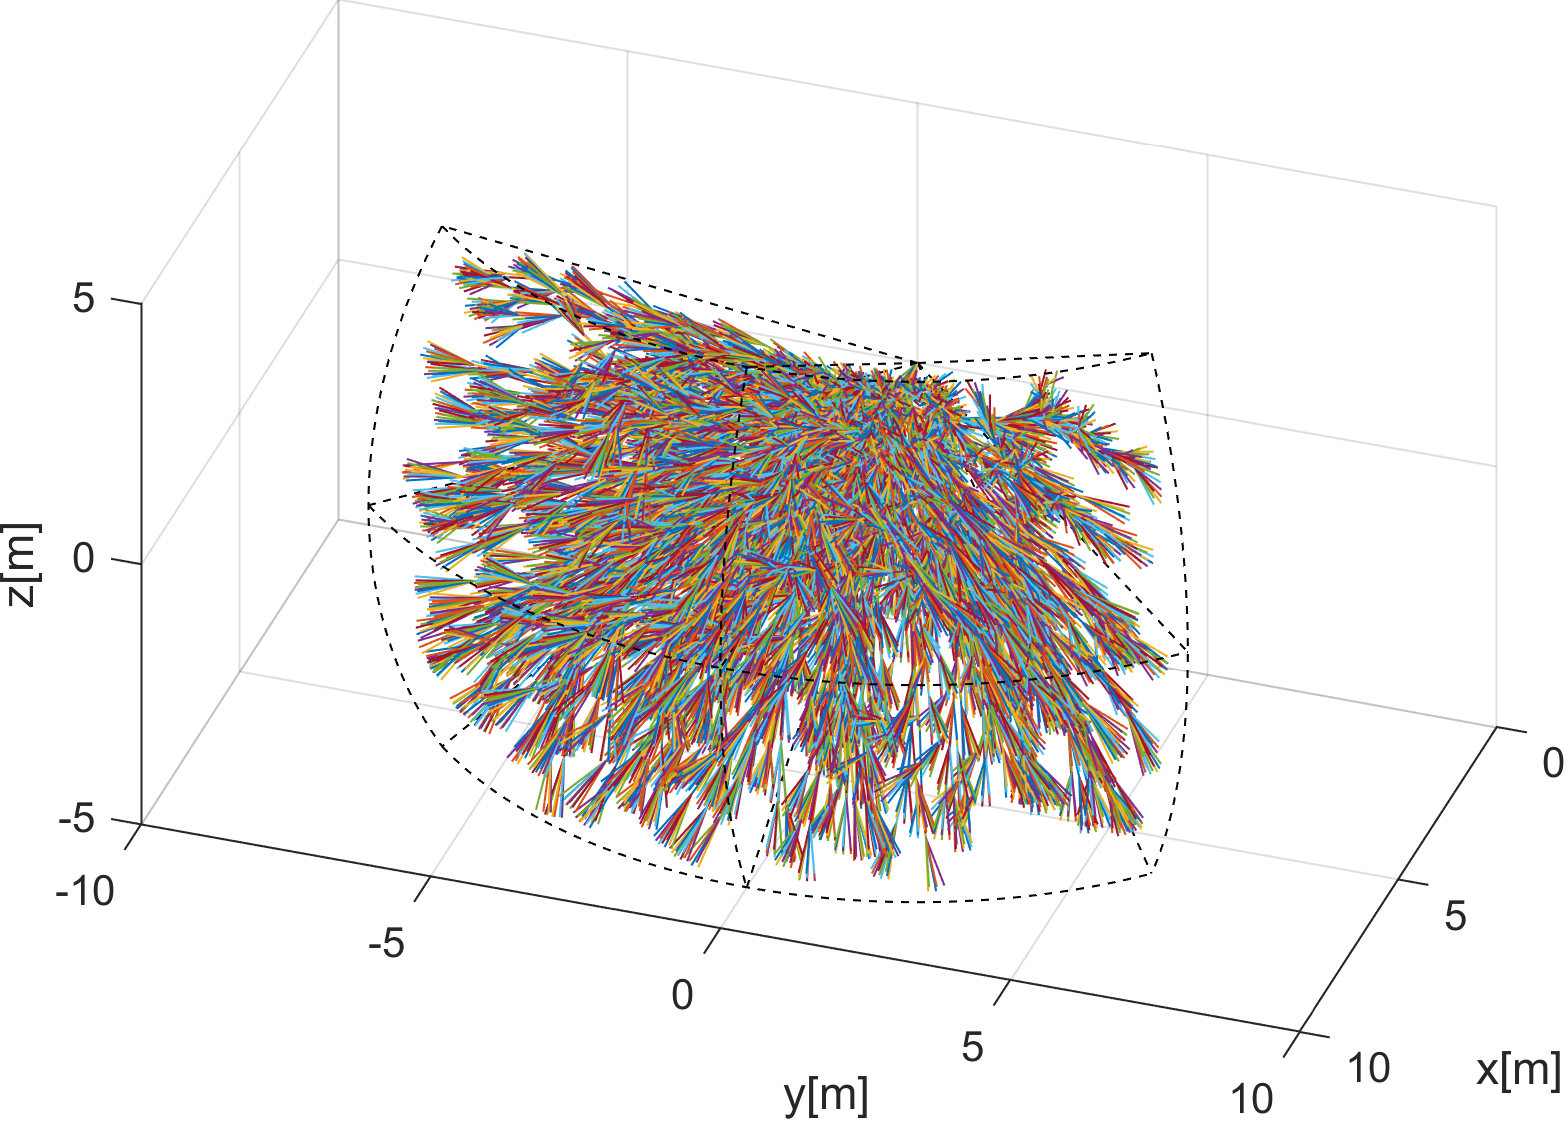
\includegraphics[width=0.9\linewidth]{\FIGDIR/NS084smoothRS00010}
        \caption{Full.}
        \label{fig:harmonicComputed}
    \end{subfigure}
    \begin{subfigure}{0.48\textwidth}
    	\centering
        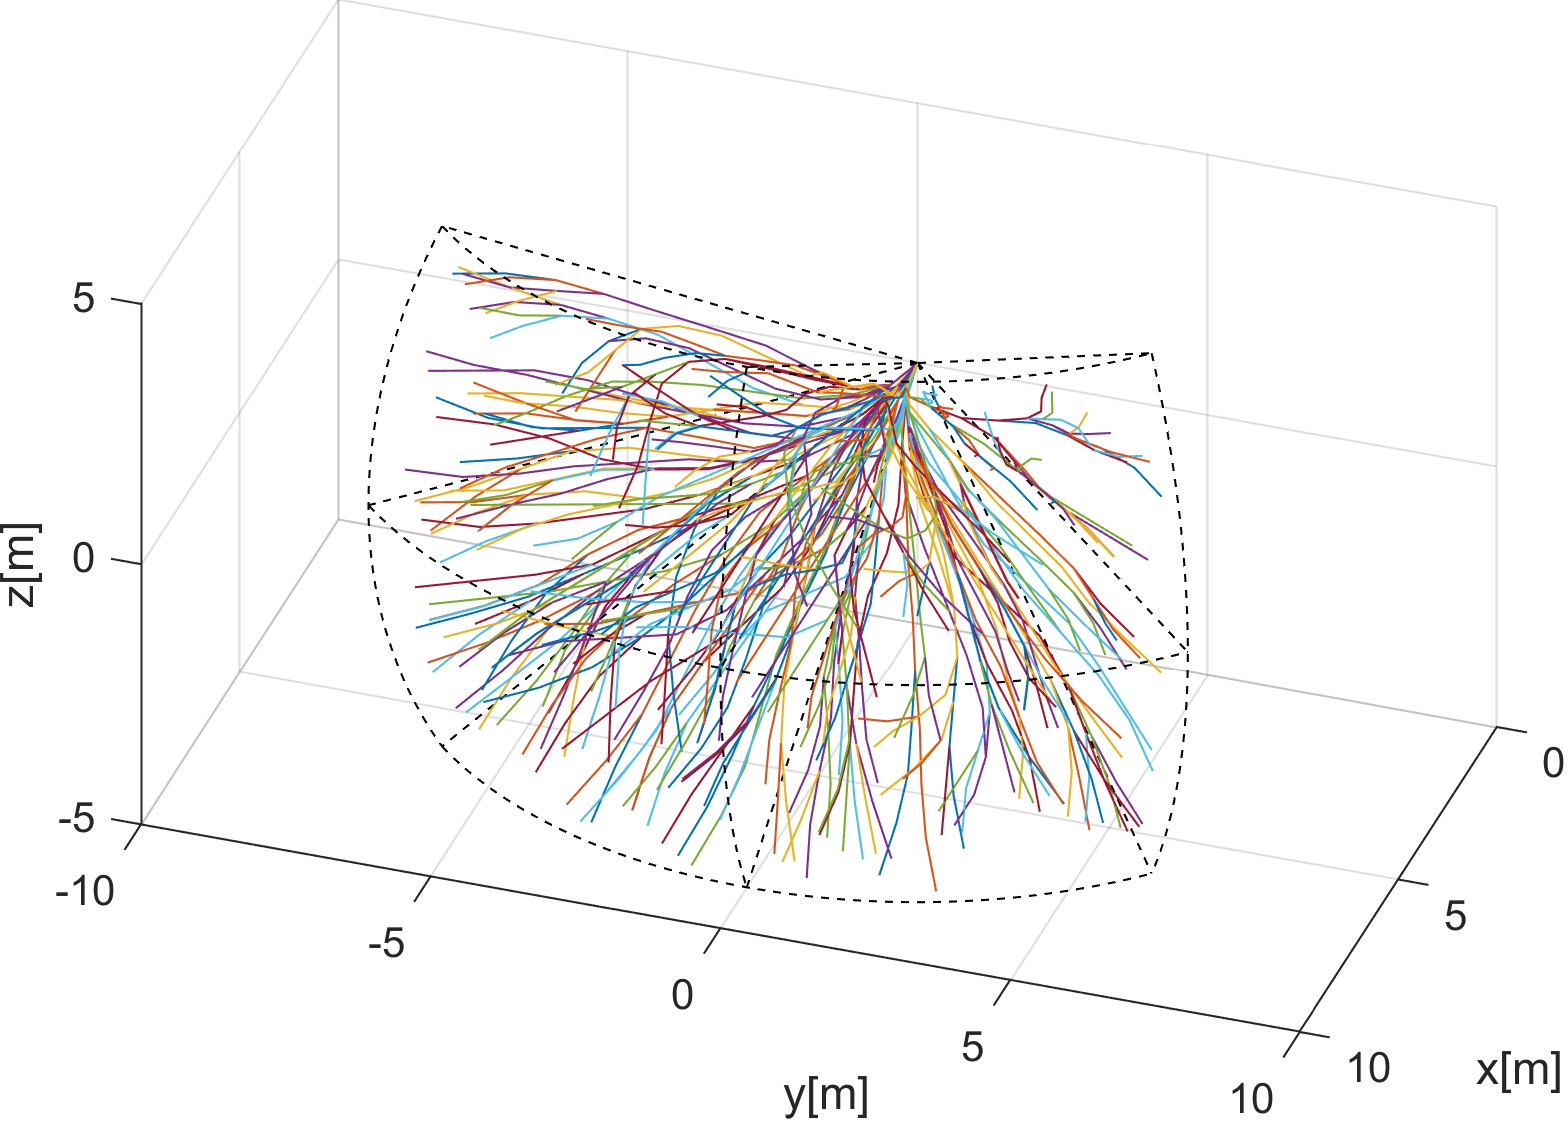
\includegraphics[width=0.9\linewidth]{\FIGDIR/NS085smoothRSAfterPruning} 
        \caption{Pruned.}
        \label{fig:harmonicPruned}
    \end{subfigure}
    \caption{Harmonic reach set computation example.}
    \label{fig:harmonicReachSetComputationExample}
\end{figure}

\paragraph{Combined Reach Set} (sec. \ref{s:combinedReachSet}) is combination of \emph{Chaotic Reach Set} (fig. \ref{fig:chaoticReachSetComputationExample}) and \emph{Harmonic Reach Set} (fig. \ref{fig:harmonicReachSetComputationExample}). The \emph{tuning parameters} are same for respective methods. It is used for both \emph{Emergency Avoidance} and \emph{Navigation}. 

\paragraph{ACAS-like Reach Set} (sec. \ref{s:acasReachSet}) is used in \emph{Navigation Mode} for \emph{Controlled Airspace}. The separations used are: \emph{Horizontal},\emph{Vertical}, \emph{Slash}, and, \emph{Backslash}, to give worst possible nodes and trajectories count. The \emph{full} set of trajectories is given in (fig. \ref{fig:acasLikeComputed}). The \emph{Pruned} set of trajectories is given in (fig. \ref{fig:acasLikePruned}).

\begin{figure}[H]
    \centering
    \begin{subfigure}{0.48\textwidth}
    	\centering
        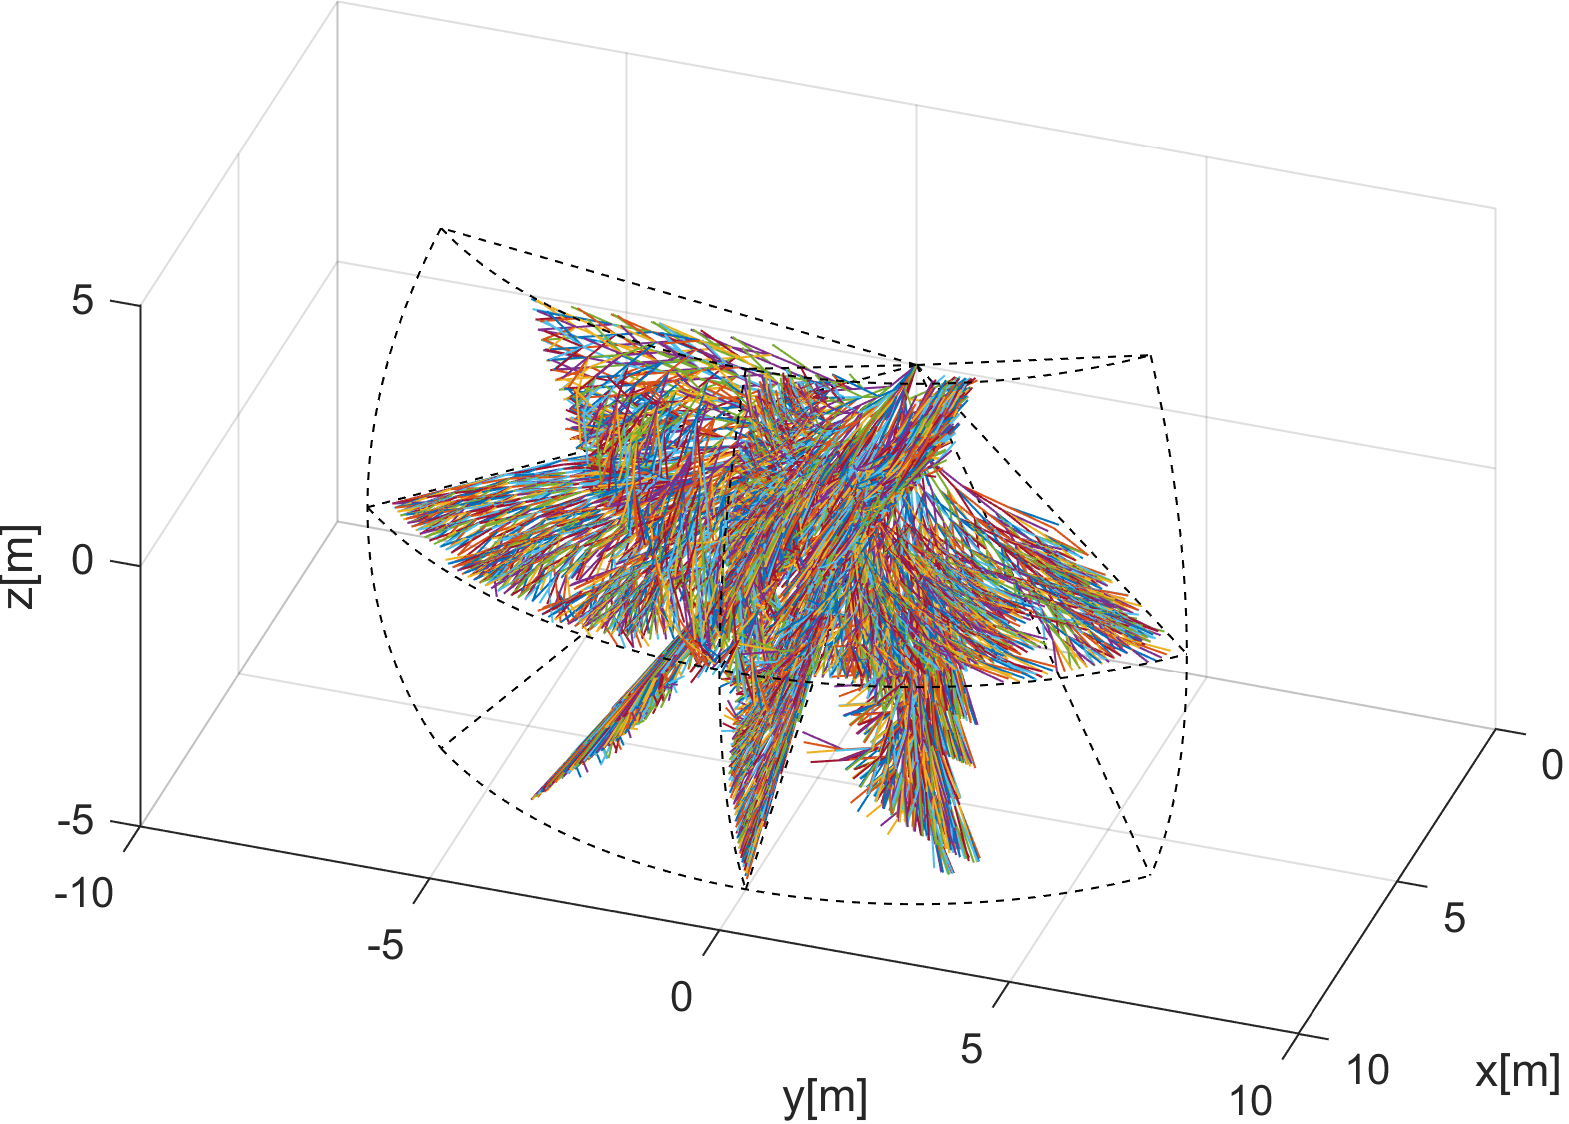
\includegraphics[width=0.9\linewidth]{\FIGDIR/NS080acasLikeRS00010}
        \caption{Full.}
        \label{fig:acasLikeComputed}
    \end{subfigure}
    \begin{subfigure}{0.48\textwidth}
    	\centering
        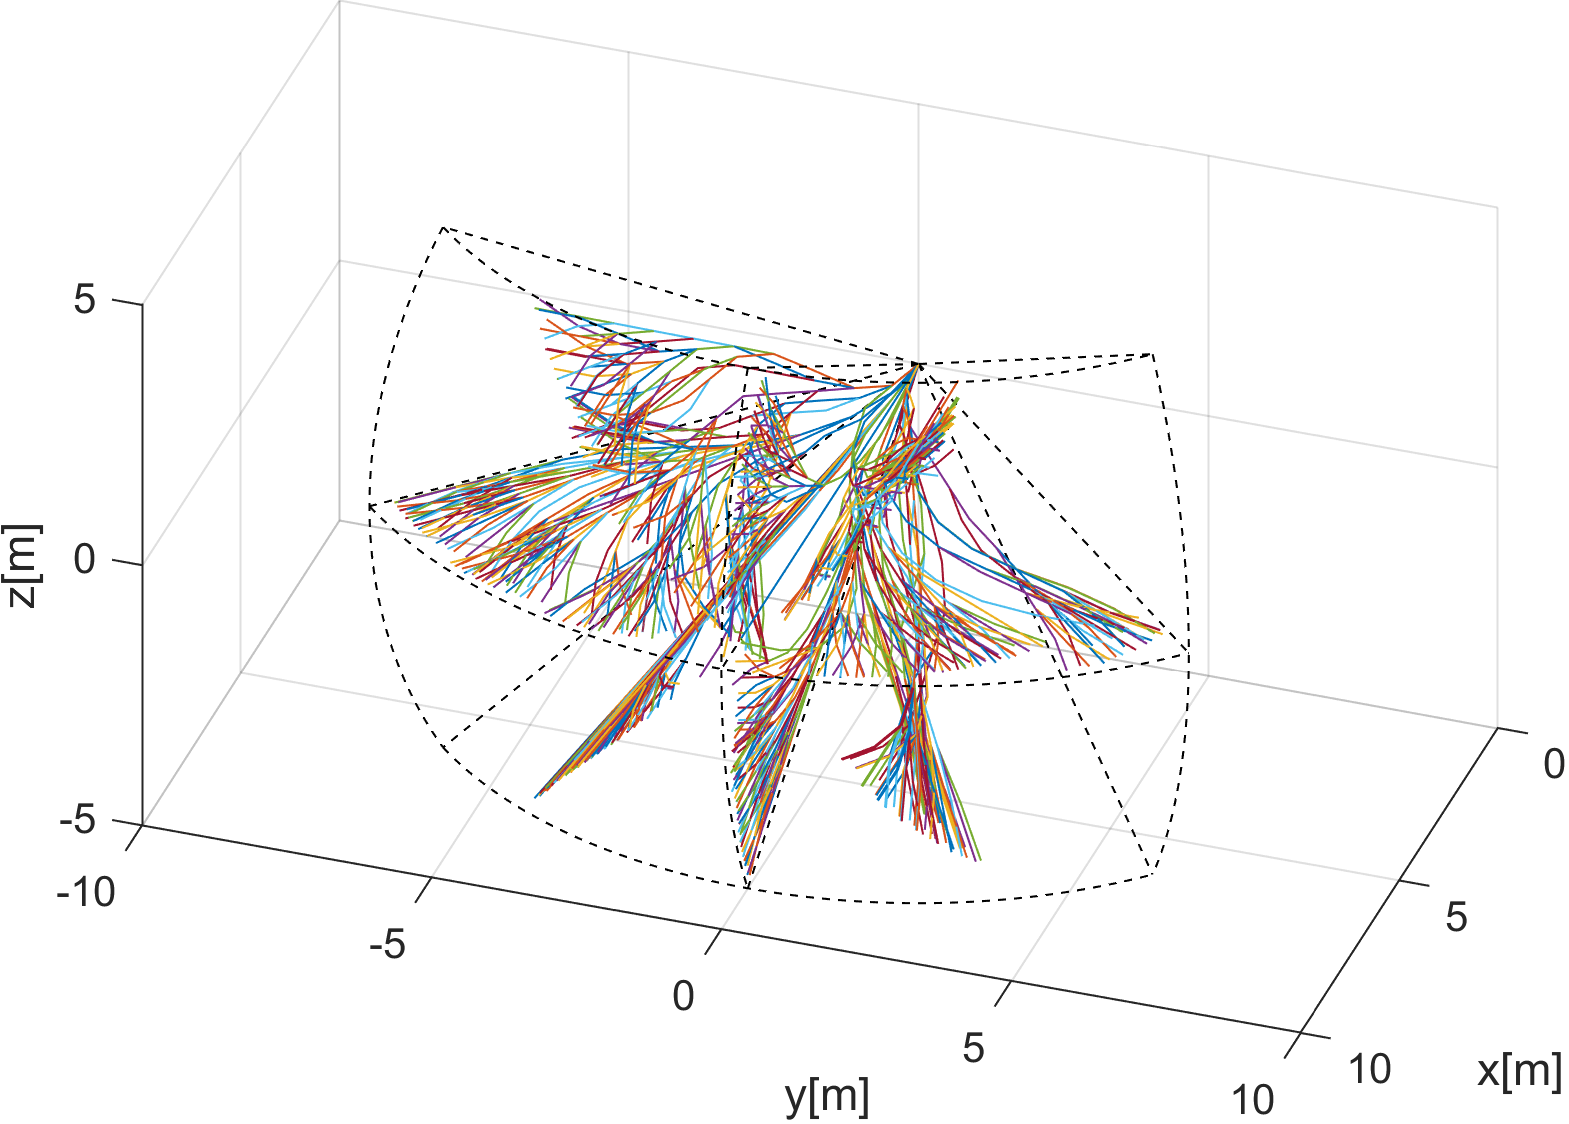
\includegraphics[width=0.9\linewidth]{\FIGDIR/NS081acasLikeRSAfterPruning} 
        \caption{Pruned.}
        \label{fig:acasLikePruned}
    \end{subfigure}
    \caption{ACAS-like reach set computation example.}
    \label{fig:acasLikeReachSetComputationExample}
\end{figure}


\paragraph{Computation Methods Performance Comparison} (tab. \ref{tab:RRMethodsPerformanceComparison})  gives overview of memory consumption and \emph{Coverage Ratio}.

\paragraph{Node count:} \emph{Full Node Count} shows how much memory it takes to compute \emph{Reach set} . \emph{Pruned Node Count} shows how much \emph{memory} is needed for storage. 

\begin{note}
    Total size of \emph{full/pruned Reach Set} depends on Node implementation. The Object oriented prototype implementation in Matlab for example avoidance grid taken up to 1 megabyte of system memory. The effective implementation would take up to 100 kilobytes.
\end{note}

\emph{Constrained expansion} (alg. \ref{alg:Wavefront Propagation}) have different selection rate, depending on method. The survival rate directly reflects strictness of selection criteria. The rate of \emph{node pruned} is summarized in (eq.\ref{eq:NodeWasteRate})  

\begin{equation}\label{eq:NodeWasteRate}
    \begin{aligned}
        \texttt{No} & \texttt{des } \texttt{pruned}\\
        &chaotic   &: 78.93 \%\\
        &harmonic  &: 18.50 \%\\
        &ACAS-like &: 79.05 \%
    \end{aligned}
\end{equation}

\noindent The \emph{interpretation or results} for each reach set estimation method is like follow: 

\begin{enumerate}
    \item \emph{Chaotic} - the main exploration drive  is \emph{Coverage Rate}, the \emph{Trajectory} segments are not usually smooth. For our \emph{Movement Automaton} there is only one \emph{Smooth Movement} : Straight. Other 8 are considered \emph{Chaotic Movements}. Impact of this fact is significant, because $4/5$ of nodes were pruned.
    
    \item \emph{Harmonic} - the main exploration drive is \emph{Smoothness} of contained \emph{Trajectories}. The \emph{Trajectory segments} which are getting further away from \emph{cell center} are not feasible. If \emph{Smooth Movements} set size is considered, the Smooth/Chaotic ratio is $1/8$ for our \emph{Movement Automaton} implementation. The low node count was expected in this approach. Other Contributing factor is \emph{Trajectory Footprint Length} for uniqueness selection, which is not a tuning parameter in this method, and it is set to most strict selection.
    
    \item \emph{ACAS-like} - the main drive is to create set consisting from \emph{multiple 2D separation planes}. The expansion method applies full movement set on \emph{candidate node}. The \emph{Separation plane movement subset} is determining, which node will be selected for further expansion. The size of separation plane subset to size of movement set rate is $1:3$. There are four separation planes: horizontal, vertical, slash and backslash each containing full 2D plane reach set approximation which caused high node prune rate. Nodes used rate should get lower with increasing grid size.
    
\end{enumerate}

\paragraph{Trajectories count:} \emph{Full trajectories count} shows how many \emph{leaf nodes} were existing during calculation process without pruning. The difference between \emph{full node count} and \emph{full trajectories count} is count of inner tree nodes. 
\emph{Pruned trajectories count} shows how many \emph{leaf nodes} are used in run-time of \emph{avoidance algorithm}. The difference between \emph{pruned node count} and \emph{pruned trajectories count} shows the count of inner nodes in active reach set.

The most of \emph{waste leaf nodes} are removed during \emph{layer pruning}: function \emph{reachSet.purge- SameFootprint()} (alg. \ref{alg:Wavefront Propagation}). The \emph{Waste trajectories} or \emph{unused leaf nodes count} have significant impact. Because \emph{leaf nodes} are side product of \emph{Node Expansion procedure} the amount of  \emph{pruned trajectories} is around 90 $\%$ regardless of the used method. The results are summarized in (eq. \ref{eq:trajectoriesWasted})

\begin{equation}\label{eq:trajectoriesWasted}
    \begin{aligned}
        \texttt{  Tr} & \texttt{ajectories } \texttt{pruned}\\
        &chaotic   &: 91.24 \%\\
        &harmonic  &: 88.21 \%\\
        &ACAS-like &: 89.43 \%
    \end{aligned}
\end{equation}

\begin{table}[H]
    \centering
    \begin{tabular}{c||c|c||c|c||c||c}
        % Header line 1
        \multirow{2}{*}{\begin{tabular}[c]{@{}c@{}}Calculation\\ method\end{tabular}} & \multicolumn{2}{c||}{Node count} & \multicolumn{2}{c||}{Trajectories} & \multirow{2}{*}{\begin{tabular}[c]{@{}c@{}}Coverage \\ ratio\end{tabular}} & \multirow{2}{*}{Parameters}\\ \cline{2-5}
        % Header line 2
        & full & pruned & full & pruned & & \\ \hline\hline
        % Chaotic reach set parameters
        chaotic  & 6727 & 1417 & 4557 & 399 & 90\% & spread:15 \\ \hline
        % Harmonic reach set parameters
        harmonic & 1724 & 1405 & 1528 & 180 & 30\%  & spread:9  \\ \hline
        % Combined reach set parameters
        combined & - & 2405 & - & 435 & 95\% & \begin{tabular}[c]{@{}c@{}}CH spread:15\\ H spread:9\\ tree comb.\end{tabular}\\ \hline
        % ACASLike
        ACAS-like & 11294 & 2366 & 7437 & 786 & 74.95\% & \begin{tabular}[c]{@{}c@{}}Separations:\\ H/V/S/BS\\ Coverage pruning:\\ disabled\end{tabular} \\ 
    \end{tabular}
    \caption{\emph{Reduced reach set} computation methods performance}
    \label{tab:RRMethodsPerformanceComparison}
\end{table}

\paragraph{Coverage ratio:} (def. \ref{def:coverageRatio}) is showing how much maneuvering versatility of \emph{Reach Set}. \emph{Full Reach Set Approximation} have coverage ratio of $100$ $\%$. It is possible to construct \emph{Reference Reach Set} without constrained expansion method which contains all possible \emph{trajectory footprints}. Following observations for \emph{coverage ratio} can be made:
\begin{enumerate}
    \item \emph{Chaotic} reach set estimation method by design select \emph{Nodes} which have probability of \emph{trajectory footprint} diversification. The high coverage ratio was achieved at values around 90 $\%$.
    
    \item \emph{Harmonic} reach set estimation method by design selects most smooth trajectories which cause low \emph{trajectory footprint} diversity. Fairly high coverage ratio of $30$ $\%$ has been achieved.
    
    \item \emph{Combined} reach set estimation method takes two reach set and combine their trajectory trees into single trajectory tree. It is given that \emph{Coverage ratio} will achieve at least maximal coverage ratio of original reach sets. Harmonic reach set supplemented narrow smooth trajectories which were throw away previously. This increased overall \emph{coverage ratio} to $95$ $\%$. 
    
    \item \emph{ACAS-like} reach set estimation method contained 4 separation planes, which caused that it was similar to \emph{Chaotic Reach Set Approximation} for given \emph{Avoidance Grid}, in terms of performance. The coverage ratio For 2D plane was $100$ $\%$.
\end{enumerate}

